\chapter{System Architecture}
\label{ch:architecture}

\section{Overview}
\label{sec:arch-overview}

MedAdhere sends an enrolled patient a short check-in text at each scheduled
dose time. The patient replies in their own words, with no required keywords or
menu codes. A large language model classifies the reply into a structured
adherence record, and a clinician dashboard shows adherence timelines, trends,
alerts, and review queues built from those records.
Figure~\ref{fig:arch-overview} shows the loop, and this chapter follows it in
order.

The platform runs on Amazon Web Services (AWS), with Twilio for SMS and the
Anthropic Messages API for the language model. Every AWS resource is declared
in AWS CDK (Cloud Development Kit) TypeScript, so one stack definition creates
and destroys the whole environment. Reliability, security, and privacy targets
are research-grade, and the design favours simplicity, auditability, and clean
teardown over high availability.

\begin{figure}[htbp]
  \centering
  \resizebox{\textwidth}{!}{%
  \begin{tikzpicture}[
    box/.style={draw, rounded corners, align=center, minimum width=2.7cm,
      minimum height=0.9cm, fill=medDetFill, draw=medDetLine},
    external/.style={box, fill=medExtFill, draw=medExtLine},
    store/.style={draw, cylinder, shape border rotate=90, aspect=0.25,
      align=center, minimum width=2.6cm, minimum height=1.1cm, fill=medStoreFill,
      draw=medStoreLine},
    flow/.style={-{Latex[length=2.4mm]}, thick, medInk},
    async/.style={flow, dashed}
  ]
    \node[external] (patient) at (-4.2,0) {Test patient\\SMS phone};
    \node[external] (twilio) at (0,0) {Twilio\\SMS + webhooks};
    \node[box] (inbound) at (4.2,0) {API Gateway\\+ Inbound Lambda\\verify, store, publish};
    \node[box] (classifier) at (8.4,0) {Classifier Lambda\\attribute + classify\\safety layer};
    \node[external] (anthropic) at (12.6,0) {Anthropic\\Messages API};

    \node[box] (scheduler) at (4.2,2.4) {EventBridge Scheduler\\dose + timeout\\one-shots};
    \node[box] (workers) at (8.4,2.4) {Outbound / Timeout\\Lambdas\\send or record};

    \node[external] (clinician) at (-4.2,-2.4) {Researcher /\\clinician view};
    \node[external] (dashboard) at (0,-2.4) {Vercel dashboard\\Cognito login};
    \node[box] (dataapi) at (4.2,-2.4) {JWT-authorized\\data API Lambda};
    \node[store] (rds) at (8.4,-2.4) {RDS PostgreSQL\\operational data};

    \draw[flow] (patient) -- node[above]{reply} (twilio);
    \draw[flow] (twilio) -- (inbound);
    \draw[async] (inbound) -- (classifier);
    \draw[flow] (classifier) -- (anthropic);
    \draw[flow, bend left=25] (anthropic) to (classifier);

    \draw[flow] (scheduler) -- (workers);
    \draw[flow] (workers.east) -- ++(0.55,0) |- (rds.east);
    \draw[flow] (inbound) -- (rds);
    \draw[flow] (classifier) -- (rds);
    \draw[flow] (dataapi) -- (rds);
    \draw[flow] (dashboard) -- (dataapi);
    \draw[flow] (clinician) -- (dashboard);

    \node[draw=medSlate, dashed, rounded corners, fit=(scheduler)(workers)(inbound)
      (classifier)(dataapi)(rds), inner sep=0.35cm,
      label={[font=\bfseries]above:AWS CDK stack}] {};
  \end{tikzpicture}}
  \caption{High-level MedAdhere architecture and the main message and read
  paths. Third-party APIs and the dashboard host remain outside the CDK stack.}
  \label{fig:arch-overview}
\end{figure}

\section{Infrastructure and Network}
\label{sec:arch-iac}

The repository is an npm-workspaces monorepo with four TypeScript packages:
\texttt{infra/} (CDK), \texttt{backend/} (Lambda handlers on Node.js ARM64),
\texttt{dashboard/} (Next.js), and \texttt{packages/shared/} (types, enums, and
schemas shared by all of them). All AWS resources live in one CDK stack, so one
\texttt{cdk deploy} brings the system up and one \texttt{cdk destroy} removes
it. Every stateful resource is declared with \texttt{RemovalPolicy.DESTROY} and
\texttt{deletionProtection} disabled by default, because the AWS defaults would
leave an orphaned database running after a ``successful'' destroy. A single
context flag inverts that setting for a live window. Assertions against the
synthesized CloudFormation template catch deploy-time errors without touching a
live account.

Every Lambda that touches the database, including the Inbound webhook Lambda,
runs in private subnets across two availability zones. Egress to third-party
APIs goes through a single NAT gateway, since none of those endpoints offers
AWS PrivateLink. An interface endpoint for Secrets Manager serves the database
credentials and the Anthropic API key at invoke time, and a gateway endpoint
for S3 keeps high-volume AWS traffic off the NAT gateway. The NAT gateway
dominates steady-state cost, so the stack runs for a working window and is
torn down afterwards, with the teardown verified.

\section{Data Model}
\label{sec:arch-data}

Persistence is a single RDS PostgreSQL~16 instance (\texttt{db.t4g.micro},
Single-AZ). One idempotent \texttt{schema.sql} defines it. A schema-init Lambda
applies it at deploy time, and integration tests apply it twice against a real
PostgreSQL container to prove it re-applies cleanly.

Seven tables carry the scheduled check-in domain: \texttt{patient} (identity,
phone number, medication, timezone, the frozen drug profile of
Section~\ref{sec:arch-drug}, and an \texttt{is\_test} flag for test-data
isolation), \texttt{dose\_schedule}, \texttt{outbound\_message} (Twilio message
SID and a forward-only delivery status, kept by a rank-guarded update that
ignores late, out-of-order callbacks), \texttt{inbound\_reply} (raw text, the
SID used for webhook deduplication, late and safety flags),
\texttt{adherence\_record}, \texttt{safety\_events}, and \texttt{label\_match}.
The conversational agent adds the append-only \texttt{clinical\_event} log and
the durable \texttt{information\_need} table of
Chapter~\ref{ch:conversational}. The classification enums are PostgreSQL enum
types whose values are defined once in \texttt{packages/shared} as a Zod
schema. The database, classifier, evaluation harness, and dashboard therefore
share one label vocabulary, and each boundary converts input into a typed value
or rejects it~\cite{king2019parse}.

Three write rules matter for correctness. \texttt{adherence\_record} has a unique constraint on
\texttt{dose\_id} and records who decided it. The timeout path inserts with
\texttt{ON CONFLICT DO NOTHING}, and the classifier upserts but may only
overwrite a timeout-decided row. A late reply can therefore correct a
provisional ``missed'' record, and nothing can overwrite a classifier decision.
\texttt{clinical\_event} is append-only: a correction inserts a new row that
supersedes the old one. Every child table references \texttt{patient} with
\texttt{ON DELETE CASCADE}, so one
\texttt{DELETE FROM patient WHERE is\_test = true} transaction removes all test
data. The same mechanism serves per-person deletion on request and teardown.

\section{Outbound Pipeline}
\label{sec:arch-outbound}

Dose scheduling uses EventBridge \emph{Scheduler} one-shot schedules instead of
cron-style Rules (Section~\ref{sec:arch-decisions}), with
\texttt{ActionAfterCompletion: DELETE} so each schedule deletes itself after
firing. Each schedule name starts with the patient identifier, a prefix that
survives the service's 64-character truncation. The service has no
prefix-delete operation, so deactivation lists the patient's schedules by
prefix, page by page, and deletes each one. A local dose time is combined with
the patient's IANA timezone and converted to the absolute UTC instant at which
the entry fires.

The Outbound Lambda renders the check-in body from a single Mustache template
and sends it through the Twilio REST API. Idempotency comes from a
\emph{pre-send reservation}. The Lambda first inserts an
\texttt{outbound\_message} row in state \texttt{sending} with
\texttt{ON CONFLICT (dose\_id) DO NOTHING} and skips the send if no row was
inserted, so a second invocation for the same dose cannot send. This turns an
at-least-once trigger into an at-most-once effect~\cite{helland2012idempotence}.
A read-then-check design cannot do that when a Twilio send succeeds and the
following database write fails. The reservation covers only the per-dose
check-in; conversational follow-ups carry their own guards
(Chapter~\ref{ch:conversational}). Delivery receipts arrive on a separate
status-callback endpoint. Its only authentication is Twilio's HMAC-SHA1 request
signature, validated over the exact configured callback URL and the full
parameter set. The route has no other authorizer because Twilio cannot present
one.

\section{Inbound Pipeline}
\label{sec:arch-inbound}

The inbound webhook is an API Gateway HTTP API (v2) endpoint backed by the
Inbound Lambda. Twilio imposes a hard timeout on webhook responses, so the
handler returns well under it even on a cold start, and no language-model call
happens on this path. Every step is safe under
redelivery. The handler first validates the \texttt{X-Twilio-Signature}
HMAC over the full parameter set and the pinned public URL, before any side
effect. It then deduplicates on the Twilio \texttt{MessageSid}. It handles
\texttt{STOP} inline by deactivating the patient and deleting all their future
schedules, reconciled with Twilio's own opt-out handling and paired with a
configured \texttt{HELP} auto-reply. Finally it stores the raw reply as an
\texttt{inbound\_reply} row and enqueues it on the patient-keyed FIFO work
queue before returning empty TwiML.

Separating the Inbound and Classifier Lambdas is \emph{bulkhead
isolation}~\cite{nygard2018releaseit}. The webhook path must be fast and
simple, while classification makes an external LLM call with retries and
multi-second latency. The FIFO queue delivers one message per invocation, so
one patient's replies are never processed concurrently. Crash-class failures on
the asynchronous leg drain to dead-letter queues with depth alarms.

\section{The LLM Classifier}
\label{sec:arch-classifier}

The Classifier Lambda turns free-text replies into structured records. This
section describes it as evaluated in Chapter~\ref{ch:results}. In the deployed
system the conversational turn processor of Chapter~\ref{ch:conversational}
takes its place and writes the same record under the same contract. The
classifier first attributes the reply to a dose: the most recent outbound
message for that patient whose dose has no classifier-decided record and whose
send time falls within the response window plus a late allowance (24 hours by
default). Replies that match no dose are stored unattributed and shown in a
review queue.

The model call goes directly to the Anthropic Messages API with the bare model
id \texttt{claude-haiku-4-5-20251001} and a \emph{forced tool}. The request
declares exactly one tool, whose JSON input schema is derived from the shared
Zod classification schema, and pins \texttt{tool\_choice} to that tool, so the
model cannot answer in prose. This is the hosted form of constrained generation (Chapter~\ref{ch:background}). The shared schema's strict
\texttt{.parse()} gate then checks the response before anything is written, so
downstream code only handles classifications that have proven their shape. The
result has two independent axes plus a safety signal:

\begin{itemize}
  \item \texttt{adherence\_state} $\in$ \{\texttt{taken},
    \texttt{delayed}, \texttt{skipped}, \texttt{stopped},
    \texttt{question}, \texttt{unknown}\}: what happened with the dose,
    mapped onto the implementation and discontinuation phases of the
    ESPACOMP ABC adherence taxonomy~\cite{vrijens2012taxonomy,
    degeest2018emerge};
  \item \texttt{reason\_code} $\in$ \{\texttt{none},
    \texttt{side\_effect}, \texttt{ran\_out}, \texttt{forgot},
    \texttt{other}\}: why, labeled on its own axis instead of folded into
    the state;
  \item \texttt{safety\_flag} $\in$ \{\texttt{none},
    \texttt{acute\_physical}, \texttt{crisis},
    \texttt{medical\_question}\}: a four-value enum instead of a boolean,
    because the safety layer branches differently on each non-none value.
\end{itemize}

Ambiguity is a valid outcome. Patients are never asked to self-classify, the
schema rewards an honest \texttt{unknown} over a forced guess, and unknowns go
to a human review queue. The prompt treats the patient's text as data. It wraps
the text in delimiter tags marked as content to classify, never as
instructions, and truncates it. The delimiters are static, so a reply that
guessed one could in principle forge a boundary. The strict parse gate and the
single permitted tool limit what such a reply could achieve, and the
adversarial gold-set slice measures the result. API failures retry with backoff
and jitter. If retries run out, the classifier writes a terminal
\texttt{unknown} record with the raw text preserved, so a transient outage
becomes a visible, reviewable row instead of a hidden dead-letter message.

\section{Safety Layer}
\label{sec:arch-safety}

A system that invites free-text replies about medication has a duty of care,
because someone may text back that they are in trouble. The safety layer is
simple and always on. Two detectors are OR'd together: a deterministic regex
prefilter over an acute-physical-symptom and crisis-signal lexicon (shared with
the evaluation harness), and the classifier's own \texttt{safety\_flag}. The
prefilter runs before the model call and can divert on its own, so an LLM
failure cannot lose a lexicon-matched emergency. This is a \emph{fail-safe
default}~\cite{saltzer1975protection}: without a working model, the system
still takes the protective path.

When either detector fires \texttt{acute\_physical} or \texttt{crisis}, the
system sends a fixed auto-reply directing the patient to emergency services
(911) or the mental-health crisis line (9-8-8) and to the researcher contact.
It records the event in \texttt{safety\_events} with a send-once upsert, so two
detectors firing produce one reply and one audit row, and it marks the reply so
that the classifier evaluation reports safety items separately. A
\texttt{medical\_question} flag takes a softer branch: an auto-reply pointing
to a pharmacist or the 8-1-1 health-advice line, logged and queued for review
without an alarm. The layer does no triage, reassurance, or symptom
interpretation. A drug-aware third detector was considered and rejected, which
keeps side-effect annotation out of the safety path.

\section{Drug Side-Effect Reference Data}
\label{sec:arch-drug}

Drug side-effect reference data follows a freeze-at-enrollment rule: no Lambda
on the message hot path calls a third-party data service. At enrollment, an
offline step resolves the patient's medication name through RxNorm's
typo-tolerant approximate matching~\cite{rxnorm}. It fetches current
structured prescribing information from openFDA~\cite{openfda} (boxed-warning
presence and text, warnings, and adverse reactions) and checks that the product
exists in Health Canada's Drug Product Database~\cite{dpd}. The result is
frozen into the patient row as a JSON profile with a fetch timestamp.
Resolution failures are warn-and-disable and never fatal.

A deterministic matcher then looks for side-effect mentions. It runs strictly
after classification, never blocks, and never touches the safety path. When the
reason code is \texttt{side\_effect} or the reply text hits a hand-built
lay-synonym map (mapping phrases like ``stomach hurt'' to MedDRA preferred
terms), the matcher intersects those terms with the drug's rows in
OnSIDES~\cite{tanaka2025onsides}. OnSIDES is a peer-reviewed reference dataset,
shipped as a static CSV in a Lambda layer and keyed by the frozen RxNorm
ingredient identifier. A match writes a \texttt{label\_match} annotation that
the review queue shows as an \emph{associative} hint, never a causal claim. The
hint is elevated only when the term also appears in the drug's boxed warning or
warnings text. No match means abstention, not an error, and the dashboard shows
the openFDA disclaimer verbatim.

\section{Non-Response Detection}
\label{sec:arch-timeout}

After each successful send, the Outbound Lambda creates a second one-shot
schedule that fires at the \emph{actual} send time plus the response window.
Anchoring to \texttt{sent\_at} instead of the nominal dose time means a delayed
send does not shrink the patient's window. The Timeout Lambda it invokes is
idempotent. It inserts a \texttt{missed}, timeout-decided adherence record with
\texttt{ON CONFLICT DO NOTHING}, so the race against a concurrent reply is
harmless in either order. Late replies are accepted, flagged
\texttt{is\_late}, and may overwrite only a timeout-decided record
(Section~\ref{sec:arch-data}).

\section{Clinician Dashboard}
\label{sec:arch-dashboard}

The dashboard is a Next.js App Router application (React, with Recharts for
charts) authenticated against an Amazon Cognito user pool. Login uses the
Hosted UI with the OAuth~2 authorization-code flow and PKCE as a public client.
Edge middleware verifies the Cognito JWT, pinned to RS256 against the pool's
JWKS, on every protected route. One administrator role is enough for a project
with a single researcher-operator.

The dashboard never talks to PostgreSQL. All data access goes through a thin
internal data API: an API Gateway HTTP API whose routes are JWT-authorized
against the same Cognito pool, backed by a Lambda in the VPC private subnets
that holds the only dashboard-facing database connection
(Section~\ref{sec:arch-decisions}). This leaves one audited, authorized path to
the data and no database credential in the
dashboard~\cite{saltzer1975protection}, and a CI guard fails the build if a
PostgreSQL client ever appears in the dashboard package. The dashboard is
hosted on Vercel; the original AWS Amplify constructs remain behind a context
flag, off by default.

The patient record is organized by day. The selected day opens as one merged
thread of the messages exchanged, the clinical events recorded from them, and
the evidence attached to each. The dose timeline, outcome reasons, label-match
hints, and frozen drug-label context sit below it
(Figure~\ref{fig:dashboard-patient}). A cohort page aggregates adherence,
active patients, reply rate, and open alerts.

\begin{figure}[tbp]
  \centering
  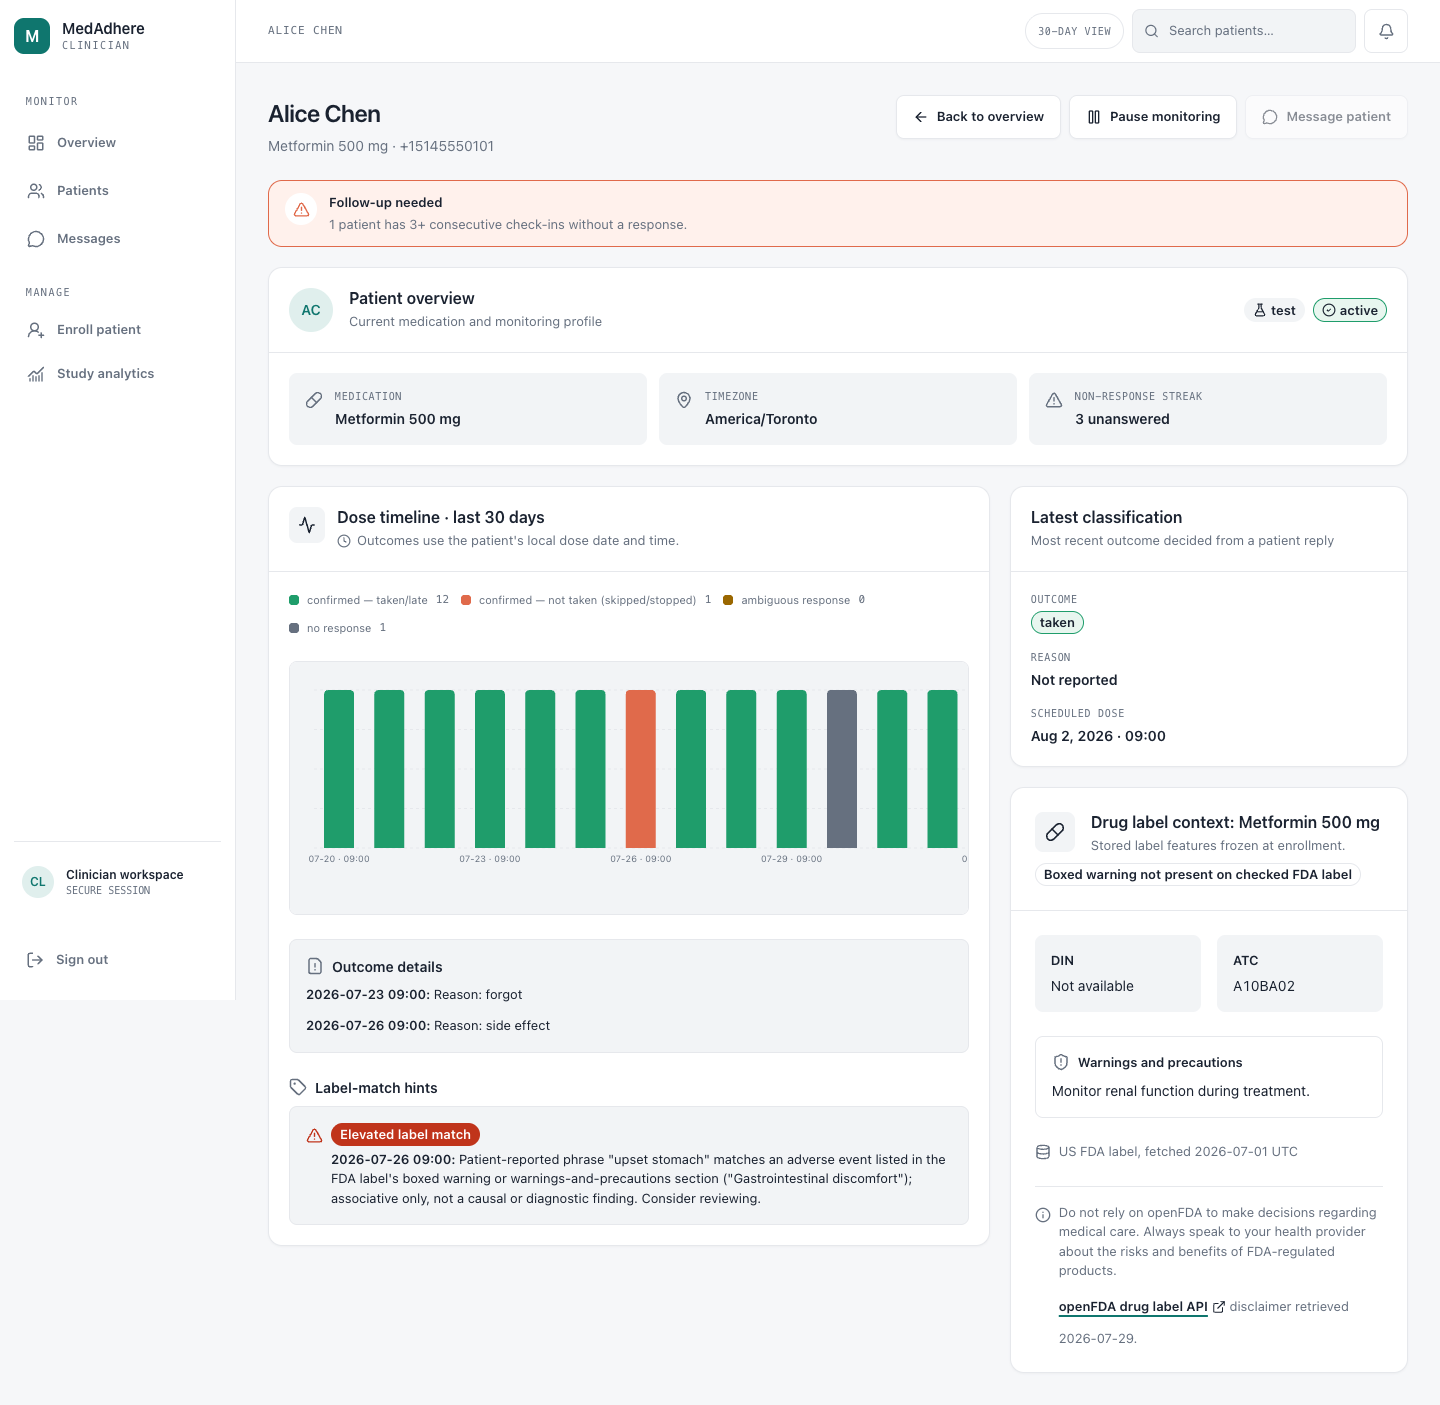
\includegraphics[width=0.75\linewidth]{figures/dashboard-patient-detail.png}
  \caption{Patient detail page for a synthetic test patient: the 30-day dose
  timeline, outcome reasons, an elevated label-match hint, and the drug-label
  context frozen at enrollment with the openFDA disclaimer. The capture
  predates the day thread, which now sits above these panels.}
  \label{fig:dashboard-patient}
\end{figure}

\section{Monitoring, Operations, and Export}
\label{sec:arch-ops}
\label{sec:arch-export}

CloudWatch alarms cover safety-event inserts, Lambda error rates,
dead-letter-queue depth, and Anthropic API failures. Budget alarms bound spend, a spend
governor puts a hard per-run cost cap on live-model evaluation runs, a
pre-deploy gate runs the regression suite before any deployment, and runbooks
cover deploy, teardown, and leak checks.

The research export is a \emph{pseudonymized} CSV for descriptive statistics.
Phone numbers become sequential pseudonyms (\texttt{patient\_}$n$), raw reply
text is excluded, and the columns are limited to what descriptive statistics
need. Pseudonymized data is not anonymous (Chapter~\ref{ch:limitations}), so
the export is paired with teardown. At project end the database, all phone
numbers, all raw reply text, and the retained final snapshot are deleted
(\texttt{cdk destroy} plus a Twilio message-log purge). Free-text evaluation
files derived from real replies stay out of version control so they remain
deletable.

\section{Key Design Decisions}
\label{sec:arch-decisions}

A concrete constraint forced each of the four decisions below.

\emph{Inference.} The plan was to call Claude Haiku 4.5 through Amazon
Bedrock. On a newly created AWS account every Bedrock token quota was
provisioned at zero, and the increase request was denied with no timeline for
reapproval. The classifier moved to the Anthropic Messages API directly, with
the same model, forced-tool contract, shared schema, and parse gate. Only one outbound
HTTPS call changed.

\emph{Scheduling.} EventBridge \emph{Rules} are recurring constructs capped at
300 per region, which a per-dose design would soon exhaust. One-shot Scheduler
entries avoid the cap at the cost of the naming convention
and paginated prefix deletion of Section~\ref{sec:arch-outbound}.

\emph{Data path and database.} Server-side rendering platforms in the
Amplify/Vercel class do not attach to a customer VPC, and the database is not
publicly reachable. Every dashboard read and write therefore goes through the
JWT-authorized in-VPC data API instead of an exposed or tunnelled database
connection. Because this predates the hosting choice, moving from Amplify to
Vercel cost only configuration. An auto-pausing serverless database engine was
rejected because it takes fifteen seconds or more to resume after a long idle
period, which pushes the first reply past Twilio's webhook timeout and
triggers a carrier retry; an always-on \texttt{db.t4g.micro} has no cold
start.

\emph{One environment.} For a system run by one person, a second stack would
double cost and configuration drift. One deployment serves testing and live
validation, with test data isolated by the \texttt{is\_test} flag.
